In this chapter, we present work in which experimentally-measured
\ac{US} pulses are used to simulate \ac{US} contrast agent microbubble
dynamics. The pulses were previously used in experiments to determine
capillary breaching thresholds in rat kidneys \citep{Miller2008b}. We
compare the calculated bubble dynamics to the
experimentally-determined bioeffects thresholds to investigate the use
of theoretical \ac{IC} thresholds as a predictor for bioeffects. This
work was published in the Journal of the Acoustical Society of America
\citep{Patterson2012, Patterson2012a}.

\section{Abstract}
  To predict bioeffects in contrast-enhanced diagnostic and
  therapeutic ultrasound procedures, the dynamics of cavitation
  microbubbles in viscoelastic media must be determined.  For this
  theoretical study, measured 1.5-7.5 MHz pulse pressure waveforms,
  which were used in experimental determinations of capillary
  breaching thresholds for contrast-enhanced diagnostic ultrasound in
  rat kidney, were used to calculate cavitation nucleated from
  contrast agent microbubbles.  A numerical model for cavitation in
  tissue was developed based on the Keller-Miksis equation (a
  compressible extension of the Rayleigh-Plesset equation for
  spherical bubble dynamics), with a Kelvin-Voigt constitutive
  relation. From this model, the bubble dynamics corresponding to the
  experimentally obtained capillary breaching thresholds were
  determined. Values of the maximum radius and temperature
  corresponding to previously determined bioeffect thresholds were
  computed for a range of ultrasound pulses and bubble sizes for
  comparison to inertial cavitation threshold criteria.  The results
  were dependent on frequency, the gas contents, and the tissue
  elastic properties.  The bioeffects thresholds were above previously
  determined inertial cavitation thresholds, even for the tissue
  models, suggesting the possibility of a more complex dosimetry for
  capillary injury in tissue.

\acresetall

\section{Background \& Introduction}
\label{sec:usbe_bubble_intro}

Cavitation-bubble collapse has been a topic of interest in physical
acoustics for nearly a century and has been the object of many
experimental and theoretical studies, which have outlined the
complexity of the phenomenon \cite[]{Leighton1997}.  This field made a
landmark contribution to non-ionizing radiation biology in medicine in
the 1980s when the possibility of inertial cavitation, with potential
induction of bioeffects, from diagnostic ultrasound pulses was
predicted theoretically \cite[]{Flynn1982,Apfel1982}.  This
possibility was included in considerations for the regulation of the
ultrasound output of diagnostic machines.  \cite{Apfel1991} performed
detailed calculations of the response of different nuclei sizes in
the form of free air microbubbles and found that the optimum size
decreased with increasing frequency, $f$.  In addition, the
rarefactional pressure amplitude threshold, $p$, for inertial
cavitation was determined for the optimum nuclei, using the criterion
of a $>$5,000 K gas temperature at collapse.  For nuclei in blood, the
ratio of $p^{1.67}/f$ was found to have a constant value of 0.13 at
the threshold, using units of MPa and MHz.  This finding was used to
create a Mechanical Index (MI) for regulatory purposes and for display
on the screens of diagnostic ultrasound machines.  The MI was set
equal to the peak rarefactional pressure amplitude (PRPA) adjusted for
attenuation and divided by the square root of frequency.  The
regulatory guideline limit for diagnostic ultrasound was considered
according to the Medical Device Amendment Act of 1976 and the maximum
value existing at that time.  This guideline limit was eventually set
from measurements on a single diagnostic ultrasound probe to be 1.9
\cite[]{Nyborg2001}.  It is noteworthy that the critical value
corresponding to the \cite{Apfel1991} result would be
\textbf{$p/f^{0.6}=0.29$}, which is much less than the MI limit.  This
discrepancy does not appear to be of concern for normal diagnostic
ultrasound from both experimental \cite[]{Carstensen2000} and
theoretical \cite[]{Church2002} considerations.

To improve diagnostic information in ultrasound examinations,
ultrasound contrast agents (UCAs) were invented.  The contrast agents
consist of a suspension of stabilized gas-filled microbubbles, which
provide strong echoes from blood and improve contrast in sonography
\cite[]{Averkiou2003, Raisinghani2004}.  Soon after contrast-enhanced
diagnostic ultrasound was developed, microscale bioeffects were
reported \citep{Miller2008a}.  The typical bioeffect seen in
mesentery, muscle, heart, and kidney was capillary rupture, which
appeared to be caused by cavitation nucleation in blood from the
circulating contrast microbubbles.  Recently, hemorrhage of glomerular
capillaries was studied in rat kidney to determine PRPA thresholds and
the frequency dependence of the thresholds \citep{Miller2008b}.
Presumably, the thresholds correspond to the action of the optimum
cavitation nuclei, and this approach therefore provides a means to
directly compare cavitation theory with the bioeffects experiments.
Over the 1.5-7.5 MHz frequency range tested, the thresholds were
proportional to the frequency, such that $p/f$ was approximately
constant at 0.49 MPa/MHz for actual diagnostic ultrasound and 0.62
MPa/MHz for diagnostic ultrasound simulated by a laboratory
pulsed-ultrasound system.  These thresholds fell below the MI=1.9
level, especially for the lower frequencies, but above the inertial
cavitation thresholds of \cite{Apfel1991}, and the frequency
dependence was different.  Evidently, the bioeffects thresholds depend
on cavitation dynamics not specifically tied to the inertial
cavitation threshold of free air bubbles in blood determined by
\cite{Apfel1991}.  The fundamental reason for these results remains
uncertain, which revives the non-ionizing radiation biology problem of
ultrasonic cavitation in medical ultrasound.

The theoretical model of \cite{Apfel1991} applies to air microbubbles
in a Newtonian liquid. However, contrast agents in the blood stream do
not necessarily exhibit such properties. It is well-known that human
tissue behaves in a viscoelastic fashion
\cite[]{Frizzell1976,Madsen1983}. The bubble dynamics greatly depend
on not only the viscoelastic properties \cite[]{Allen2000a,Yang2005}
for a given model, but also on the type of model \cite[]{Johnsen2012}
and on nonlinearity \cite[]{Allen2000b}. Furthermore, the gas
contained in contrast agents is not air; for example, perfluoropropane
(PFP, C$_3$F$_8$) in Definity (Perflutren Lipid Microsphere, Lantheus
Medical Imaging, N Billerica MA), which may affect the collapse
temperature.  The stabilizing skin or shell may not be an important
factor for the capillary rupture bioeffect because the nucleation
process appears to liberate a free gas microbubble. The thresholds for
this cavitational bioeffect are above the destabilization threshold of
the optimal microbubbles, which therefore may be modeled as free
microbubbles \cite[]{Sboros2002,Marmottant2005}.  Basically, at low
PRPAs the stabilization is lost, which releases a free microbubble,
thus nucleating cavitation, followed by dissolution at the conclusion
of the pulse \cite[]{Porter2006}.  In the case of diagnostic
ultrasound, the microbubble is subjected to a series of pulses that
start low, build to a peak and finally decline.  Thus, when the peak
pulse arrives to cause the injury, the microbubbles likely are already
destabilized.

The detailed mechanism by which cavitation causes bioeffects is
unknown, although several have been proposed, such as shock emission
upon collapse, growth beyond a given size, high temperatures
generating free radicals, re-entrant jets in non-spherical collapse
\cite[]{Nyborg2002}. In order for such phenomena to occur, it is
expected that inertial cavitation occurs. From this observation, prior
studies have used the threshold for inertial cavitation as a surrogate
for bioeffects \cite[]{Yang2005}. This inertial cavitation threshold
was developed theoretically for bubble dynamics in water
\cite[]{Flynn1975}. In this work, we show that the bioeffects
threshold is different from previously developed inertial cavitation
thresholds. The difference between the inertial cavitation threshold
calculated for air microbubbles in blood and the capillary rupture
thresholds is likely due to an incomplete model.  That is, the
homogenous model results may correlate better with the bioeffects
results if tissue elasticity, gas contents, pulse parameters, and
possibly other factors are considered.  

In the current work, a different approach combining experiments and
numerical modeling to studying bioeffects is followed.  \emph{In vivo}
experiments were performed to determine the pulse amplitude and
frequency under which bioeffects occur \cite[]{Miller2008b}.  Given
these experimental pulses, bubble dynamics are modeled numerically
over the entire waveform duration, which is not taken into account by
\cite{Apfel1991}, to determine how the bubble response correlates with
the observation of bioeffects.  A detailed description of the
methodology is presented. The experimental setup and numerical model
are first discussed in Section \ref{sec:usbe_bubble_methods}. The results
from the combined experimental and numerical procedure are presented
in Section \ref{sec:usbe_bubble_results}. The ability of established
inertial cavitation thresholds, and general cavitation parameters, to
predict bioeffects is discussed. The article ends with a summary of
the results and considerations for future work on this topic.

\section{Materials and Methods}
\label{sec:usbe_bubble_methods}
\subsection{Experimental Setup}

In the previous study of glomerular capillary hemorrhage in rats by
\cite{Miller2008b}, bioeffect thresholds were determined for
ultrasound exposure with diagnostic ultrasound machines and with a
laboratory system set up to simulate diagnostic scanning.  The
ultrasonic waveforms (pressure vs. time) used for the driving pressure
in this study were based on the laboratory system bioeffect thresholds
at 1.50, 2.25, 3.50, 5.00 and 7.50 MHz (with corresponding bioeffects
thresholds of 0.98, 1.31, 2.38, 2.82 and 6.00), which allowed more
flexibility in producing the desired pulse waveforms than the
diagnostic ultrasound machine.

The experiment was designed to simulate worst-case-scenario clinical
conditions for CEUS. Anesthetized rats were held in place in a 75 L
bath of 37$ ^\circ$ C degassed water, and exposed to ultrasound while
receiving a constant 10 $\mu$l/kg/min infusion of UCA.  The ultrasound
probe was placed such that its focal zone was at the cortex of the
right kidney.  The ultrasound system consisted of a transducer, power
amplifier (A-500, Electronic Navigation Industries, Rochester NY),
function generator (model 3314A function generator, Hewlett Packard
Co., Palo Alto CA).  Five damped single element transducers
(Panametrics, Olympus NDT Inc. Waltham, MA) with 1.9 cm diameter and
3.8 cm focus were used at their resonant ultrasonic frequencies in a
warmed water tank.  The function generator was set using the $n$-cycle
mode with $n=3$ to produce a simple pulse train with pulse durations
and PRPAs the same as used for the \textit{in vivo} exposures.  The
waveforms were measured with a calibrated PVDF bilaminar film
hydrophone with 0.4 mm spot size (model 805, Sonora Medical Systems,
Longmont CO) and were adjusted to equal the threshold at each
frequency and to several 3 dB increments above and below the
threshold.  The purpose of the progressive steps was to help identify
any specific cavity behavior, which recurred at each frequency as the
threshold was crossed.  The hydrophone measured the alternating
pressure including the PRPA, to which the constant atmospheric
pressure must be added to obtain the total pressure.  The highest PRPA
available for the higher frequencies was limited by the transducers.
The experimental waveforms are imported into Matlab, and smoothened
using a moving-average low-pass filter. This procedure results in
waveforms, such as that shown in Figure \ref{fig:waveforms} for the
threshold at 7.5 MHz, in which the high-frequency experimental noise
is removed. The smoothened waveforms are then input into the bubble
dynamics code as the driving pressure.

\begin{figure*}[!t]
  \centering 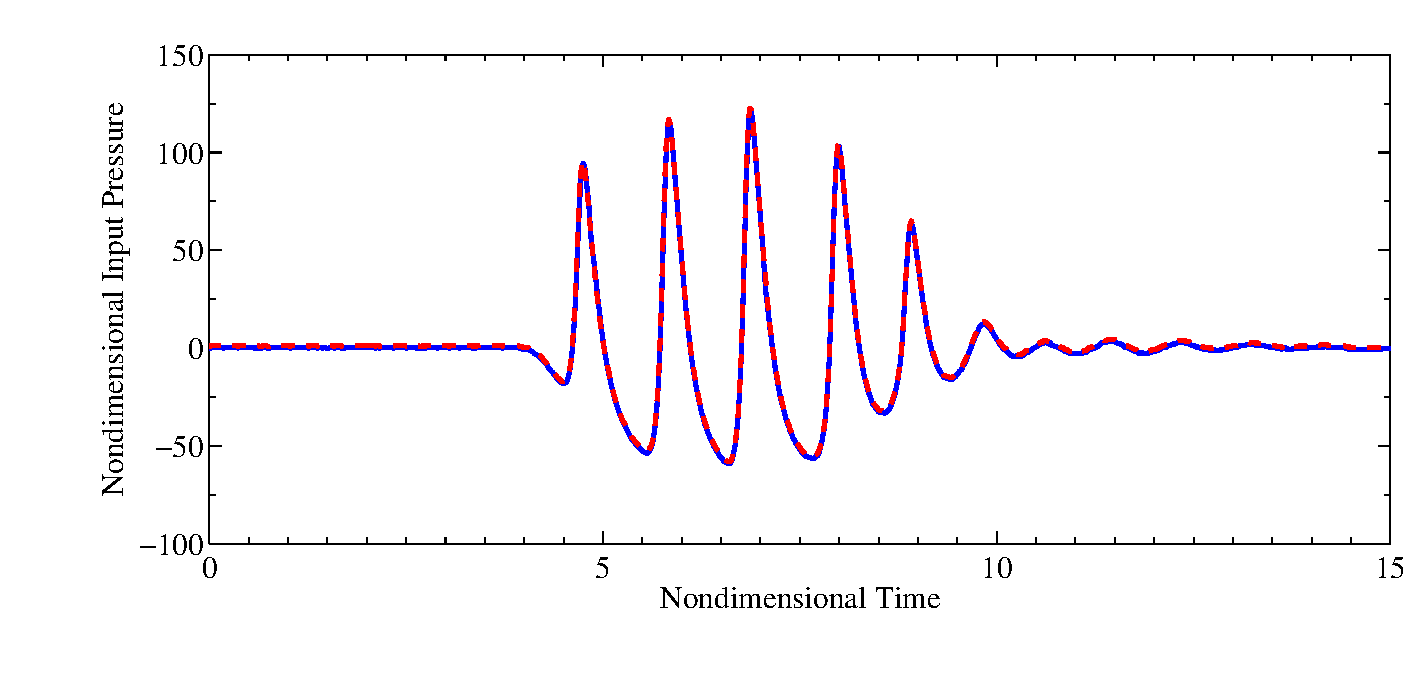
\includegraphics[width=\textwidth]{./figs/bubble_figs/PexpPsmooth}
  \caption[7.5 MHz experimental and numerical ultrasound waveforms at
  bioeffects threshold pressure]{7.5 MHz experimental and numerical
    ultrasound waveforms at bioeffects threshold
    pressure. Experimental and numerical (filtered) pressure waveforms
    for the 7.5 MHz pulse at the threshold (Peak negative pressure:
    6.0 MPa, 543 ns duration, MI$_{eq}$=PRPA/$f^{1/2}$=2.2). Solid:
    experimental; dashed: numerical.}
  \label{fig:waveforms}
\end{figure*}


\subsection{Bubble Dynamics Model}%
\label{subsec:usbe_bubble_model}%
The bubble dynamics are modeled under the assumption that a single
spherical gas bubble is subjected to a far-field pressure change
(ultrasound pulse) in an infinite medium of uniform properties.  Given
that bioeffects are observed in some of the experiments and that it is
likely that inertial cavitation occurs, it is expected that
compressibility of the surrounding medium matters. Furthermore, tissue
is expected to behave in a viscoelastic fashion. To account for all of
these elements, the Keller-Miksis equation \cite[]{Keller1980}, a
compressible extension of the Rayleigh-Plesset equation, is
considered, and the constitutive relation between the stresses and
strains follows a Kelvin-Voigt viscoelastic model, as in
\cite{Yang2005}. Thus the nondimensional equations governing the
bubble dynamics are:
\begin{eqnarray}\label{eq:keller}
  \left(1-\frac{\dot{R}}{C}\right) R \ddot{R} +
    \frac{3}{2}\left(1-\frac{\dot{R}}{3 C}\right) \dot{R}^2%\nonumber  %\\&&
     = \left(1+\frac{\dot{R}}{C}\right) \left[p_B- 1 -p_a -
    \frac{R}{C}\frac{dp_a}{dt}\right] +\frac{R}{C} \dot{p}_B,
\end{eqnarray}
where $R(t)$ is the bubble radius, $C$ is the dimensionless sound
speed, $p_a$ is the time-varying component of the far-field pressure
and the dot represents material (time) derivatives. The bubble
pressure $p_B$ is given by
\begin{align}\label{eq:bubble_pressure}
  p_B = \left(1+\frac{2}{We}\right)\frac{1}{R^{3\gamma}}-\frac{2}{We R} + \tau_R,
\end{align}
where $We$ is the Weber number (dimensionless surface tension),
$\gamma$ is the specific heats ratio for the gas, and $\tau_R$ is the
shear stress in the $rr$-direction evaluated at $r=R$.

\begin{table*}[!t]
  \centering
  \begin{tabular}{l l c l}
    Parameter & Dimensional value & & Dimensionless number \\ \hline
    Viscosity & $\mu=0.015$ (Pa s) & $\mapsto$ & $Re=\rho u R_o / \mu = 2/3$ \\
    Elasticity & $G=10^5$ (Pa) & $\mapsto$ & $Ca= \rho u^2 / G = 1.0$ 	\\
    Surface tension & $S=0.056$ (N/m) & $\mapsto$ & $We=\rho u^2 R_o / S$ = 2 \\
    Sound speed & $c=1570$ (m/s) & $\mapsto$ & $C = c/u=157$ \\  
%    Relaxation time & $\lambda = 0.5$ ($\mu$ s) & $\mapsto$ &	$De=\lambda u / R_o =0$ \\
  \end{tabular} 
  \caption{Base physical parameters representative of soft tissue used
    in the present study.}
  \label{tab:usbe_bubble_parameters}
\end{table*}


As in \cite{Yang2005}, the Kelvin-Voigt model is used as the
constitutive relation between the stresses and strains:
\begin{equation}
  \tau_R = -\frac{4}{3Ca}\left(1-\frac{1}{R^3}\right) - \frac{4}{Re}\frac{\dot{R}}{R},
\end{equation}
%\begin{equation}
%  s = \frac{4}{9
%  Ca}\left(1-\frac{1}{R^3}\right) - \frac{4}{9 Re} \frac{\dot{R}}{R},
%\end{equation}
where $Re$ is the Reynolds number (dimensionless viscosity), and $Ca$
is the Cauchy number (dimensionless elasticity).  The dimensionless
numbers are defined in Table
\ref{tab:usbe_bubble_parameters}.  %The SLS model reduces to the
%linear Maxwell model used by \cite{allen2000a} and to the linear Kelvin-Voigt
%model used by \cite{yang2005} for bubble dynamics in viscoelastic
%media in the context of medical ultrasound.
The resulting system of equations is solved for the bubble radius
using a fifth-order accurate Cash-Karp Runge-Kutta method with
adaptive time-step control. In the problem under consideration, the
pressure pulse is smooth and its wavelength is on the order of 1
mm. Since the bubbles are initially in the micron range and do not
grow beyond a few initial radii, the present Rayleigh-Plesset-type
approach is justified.

The base values for tissue properties, listed in Table
\ref{tab:usbe_bubble_parameters}, are taken from the literature
\cite[]{Apfel1991,Yang2005}. In the present work variables are
nondimensionalized using a tissue density of $\rho=1000$ kg/m$^3$, a
characteristic speed given by $u=\sqrt{p_{atm}/\rho}$ where $p_{atm}$
is atmospheric pressure, and a characteristic equilibrium radius of
$R_0=1$ $\mu$m. The resulting time scale is thus close to the Rayleigh
collapse time.  A range of equilibrium radii within 0.1-2.0 $\mu$m, a
typical size distribution for UCAs, is considered. Thus, changing the
equilibrium radius modifies the nondimensional parameters.  The
specific heat is taken as $\gamma =1.13$ for
perfluoropropane. Reported values of tissue elasticity fall in the
1-100 kPa range \cite[]{Arda2011%,maxwell2012}
}. However, it is known that the elasticity may increase up to the MPa
range at high strains \cite[]{Krouskop1998}.  Here, a nominal
elasticity of $G=100$ kPa is considered as the base case.

Since the thresholds for cavitational bioeffects are above the
destabilization threshold, the microbubbles are modeled as free
bubbles \cite[]{Sboros2002,Marmottant2005}, \textit{i.e.,} UCA
stabilizing films and shells are neglected.  Additionally, the
detailed effect of the physical constraint imposed by blood vessel
walls is considered by including it in the bulk elasticity of the
tissue. Though non-spherical perturbations may occur due to the local
heterogeneity of tissue and thus lead to a significant change in the
bubble dynamics, non-spherical collapse is expected to produce lower
temperatures and pressures \cite[]{Johnsen2009}.  In this sense, the
spherically symmetric model represents a worst-case scenario useful in
determining safe, conservative parameters for CEUS procedures.

\section{Results and Discussion}
\label{sec:usbe_bubble_results}

\subsection{Bubble Response}
Typical bubble responses are first shown to provide a qualitative
understanding of the physics.  Figures \ref{fig:sample_bubble_linear},
\ref{fig:sample_bubble_intermediate} and
\ref{fig:sample_bubble_nonlinear} show the history of the
dimensionless bubble radius produced by a given pressure waveform for
a range of essentially linear to nonlinear cases, and different
elasticities (5 kPa, 100 kPa and 1 MPa). In the linear case, the
bubble oscillations are in phase with the pressure
waveform. Increasing the elasticity leads to larger oscillation
amplitudes, though the changes are small. At intermediate frequency
and amplitude, the oscillations become larger and more nonlinear for
larger elasticities. This observation, although seemingly
counterintuitive, is consistent with the results of
\cite{Johnsen2012}, who showed analytically that the damping of the
oscillations is smaller in this range of elasticities.  In the fully
nonlinear case (large pulse amplitude and frequency), the oscillation
amplitude becomes yet larger, thus yielding a larger maximum radius
and very small minimum radius.  For all elasticities, the initial
behavior is similar up to the second maximum radius. Thereafter, the
stiffer case (G=1 MPa) departs and collapses violently, while the
other cases rebound. The maximum radius is achieved at approximately
the same time in all cases, after the peak positive pressure. In all
the simulations, the oscillations damp out rapidly after the passage
of the pulse.

\begin{figure}[!t]
  \centering 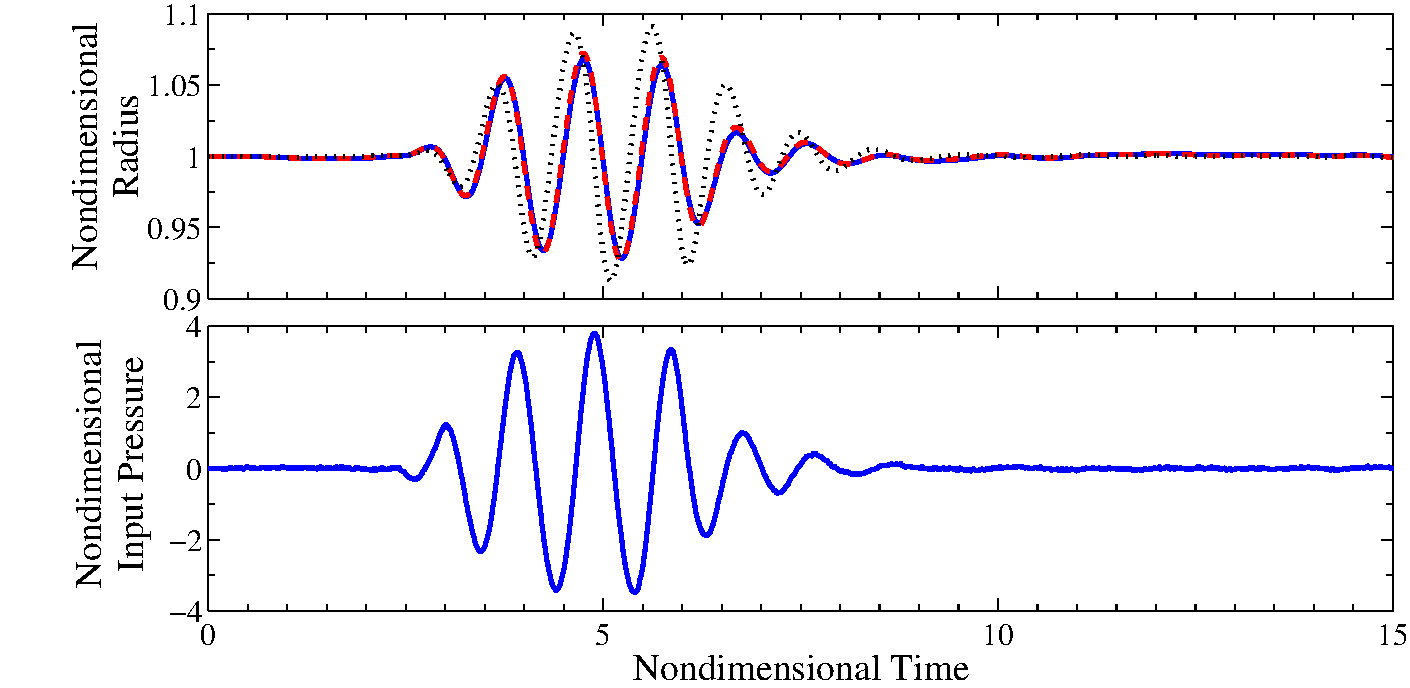
\includegraphics[width=\textwidth]{figs/bubble_figs/Rt_linear}
  \caption[Bubble radius and input-pressure
    waveform histories for an essentially linear case (frequency: 1.5
    MHz; peak negative pressure: 0.35 MPa)]{Bubble radius (top) and input-pressure
    waveform (bottom) histories for an essentially linear case (frequency: 1.5
    MHz; peak negative pressure: 0.35 MPa). No bioeffects are observed
    here. $R_0=1$ $\mu$m; solid: $G=5$ kPa; dashed: $G=100$ kPa;
    dotted: $G=1$ MPa.}
  \label{fig:sample_bubble_linear}
\end{figure}

\begin{figure}[!t]
  \centering 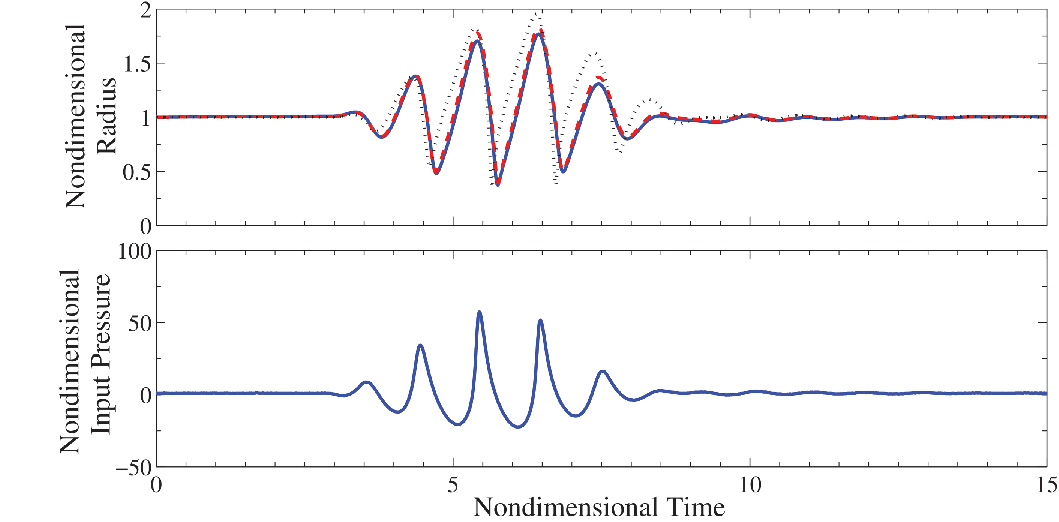
\includegraphics[width=\textwidth]{figs/bubble_figs/Rt_intermediate}%
  \caption[Bubble radius and input pressure histories for a moderately nonlinear case (frequency: 3.5
    MHz; peak negative pressure: 2.4 MPa)]{Bubble radius (top) and input-pressure
    waveform (bottom) histories for a moderately nonlinear case (frequency: 3.5
    MHz; peak negative pressure: 2.4 MPa). Bioeffects are observed
    here. $R_0=1$ $\mu$m; solid: $G=5$ kPa; dashed: $G=100$ kPa;
    dotted: $G=1$ MPa.}
  \label{fig:sample_bubble_intermediate}
\end{figure}

\begin{figure}[!t]
  \centering 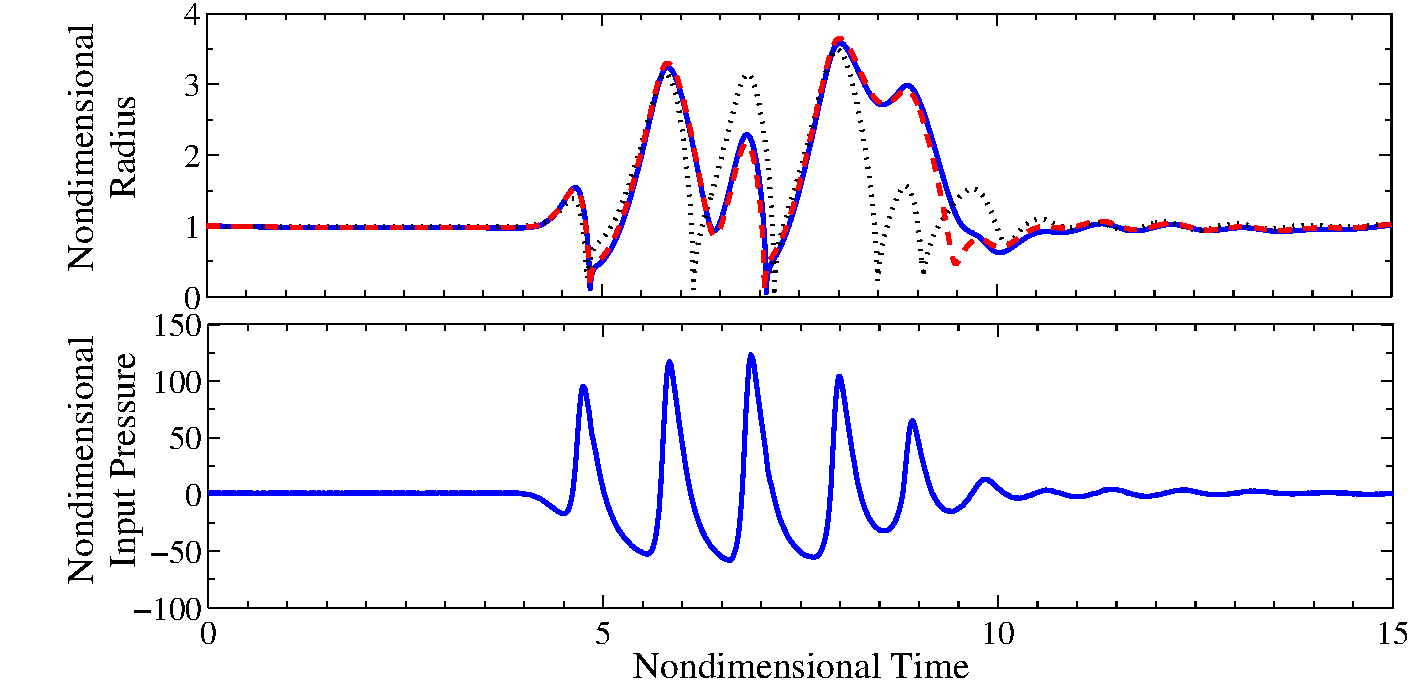
\includegraphics[width=\textwidth]{figs/bubble_figs/Rt_nonlinear}
  \caption[Bubble radius and input pressure histories for a highly nonlinear case (frequency: 7.5 MHz;
    peak negative pressure: 6.0 MPa)]{Bubble radius (top) and input-pressure
    waveform (bottom) histories for a highly nonlinear case (frequency: 7.5 MHz;
    peak negative pressure: 6.0 MPa). Bioeffects are observed
    here. $R_0=1$ $\mu$m; solid: $G=5$ kPa; dashed: $G=100$ kPa;
    dotted: $G=1$ MPa.}
  \label{fig:sample_bubble_nonlinear}
\end{figure}

In the results of the following sections, the maximum dimensionless
radius, $R_{max}$, and dimensional bubble temperature at collapse,
$T_{max}$, obtained using the ideal gas law, are determined by
recording their largest value over the simulation. These quantities
are compared to the inertial cavitation thresholds used by
\cite{Apfel1991} and \cite{Yang2005}: $R_{max}=2$ and $T_{max}=5000$
K. The dependence of the bubble dynamics on the pulse amplitude,
initial bubble size (\emph{i.e.}, UCA size distribution), pulse
frequency, and tissue properties are considered individually.



\subsection{Dependence on the Pulse Amplitude}
Given the strong dependence of the MI on the rarefactional pressure
amplitude, the influence of the pulse amplitude on the bubble dynamics
is first evaluated. Figure \ref{fig:amplitude} shows the dimensionless
maximum radius as a function of rarefactional pressure
amplitude. Initial bubble radii ranging between 0.1--2.0 $\mu$m are
shown, as well as different frequencies. The open symbols denote
cases where bioeffects did not occur, while the filled symbols denote
the occurrence of bioeffects.

\begin{figure}[t]
  \centering
  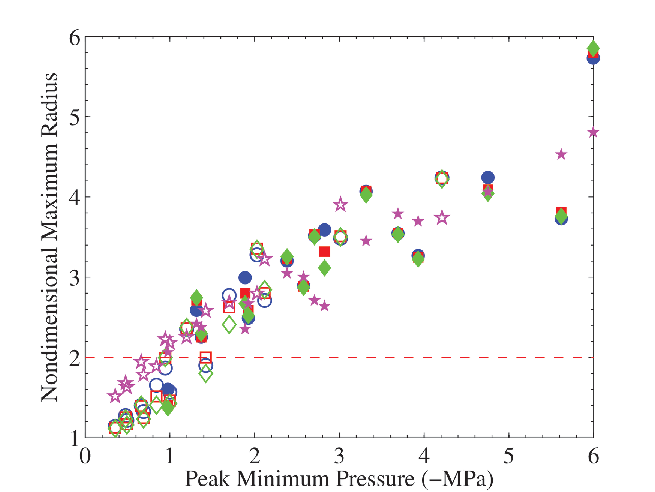
\includegraphics[width=0.7\textwidth]{figs/bubble_figs/Rstarmax_Pm}
  \caption[Dependence of the dimensionless maximum bubble radius on
  the peak negative pressure for $G=100$ kPa.]{Dependence of the
    dimensionless maximum bubble radius on the peak negative pressure
    for $G=100$ kPa.  Empty symbols: no bioeffects; filled symbols:
    bioeffects. Pentagrams: 0.1 $\mu$m; circles: 0.5 $\mu$m; squares:
    1 $\mu$m; diamonds: 2 $\mu$m; frequency: 1.5 - 7.5 MHz. The
    $R_{max}=2$ inertial cavitation threshold (red, dashed line).
  }
  \label{fig:amplitude}
\end{figure}

The results show that the bubble dynamics, through the maximum radius,
scale with the pulse amplitude. Although the results do not collapse
fully onto a line, a general trend is discernible. At low amplitude,
the increase in the maximum radius is approximately linear; beyond
some amplitude, the bubble undergoes nonlinear oscillations, thus
explaining the different dependence and larger spread.  These results
are consistent with the plots shown in
Figures \ref{fig:sample_bubble_linear}-\ref{fig:sample_bubble_nonlinear}.
Over a broad range of amplitudes, the occurrence of bioeffects has
little correlation with pulse amplitude alone: at a given amplitude,
bioeffects may be observed or not, depending on the bubble size and
pulse frequency. Only at very large pressure amplitudes (PRPA $>$
4.20 MPa) are bioeffects systematically observed regardless of the
bubble size and pulse frequency. This behavior is not surprising,
since at these amplitudes the bubble response is expected to be highly
nonlinear. Conversely, at low amplitudes (PRPA $<$ 0.97 MPa), the
oscillations are linear and no bioeffects are observed, regardless of
bubble size and pulse frequency. In this latter case, most bubbles
whose $R_{max}/R_0$ is below two do not exhibit bioeffects; however,
this behavior depends on the value of elasticity, as shown in Section
\ref{sec:usbe_bubble_tissue_properties}. Although not shown here for
conciseness, similar results are obtained for peak positive pressure.


Similarly, the criterion $T_{max} > 5000$ K is not achieved with perfluoropropane.
As shown in Figure \ref{fig:gascontents}, the observed temperatures for
PFP are far below this value, though the results for air approach it. This
result is expected since the criterion was determined for air, which
has a larger specific heats ratio ($\gamma_{air}=1.4$) than
PFP ($\gamma= 1.13$). The specific heats ratio appears in
the internal gas pressure term in Equation \ref{eq:bubble_pressure}; its
effect on the bubble dynamics is minor if the minimum radius is not
very small, as in Figure \ref{fig:gascontents}. Still, since the
adiabatic relationships for an ideal gas are used, the temperature is
significantly affected by the different specific heats ratio. Hence,
even though the bubble dynamics are not strongly affected by the
specific heats ratio, the maximum temperature is.

\begin{figure}[t]
  \centering
  \begin{subfigure}{0.47\textwidth}
    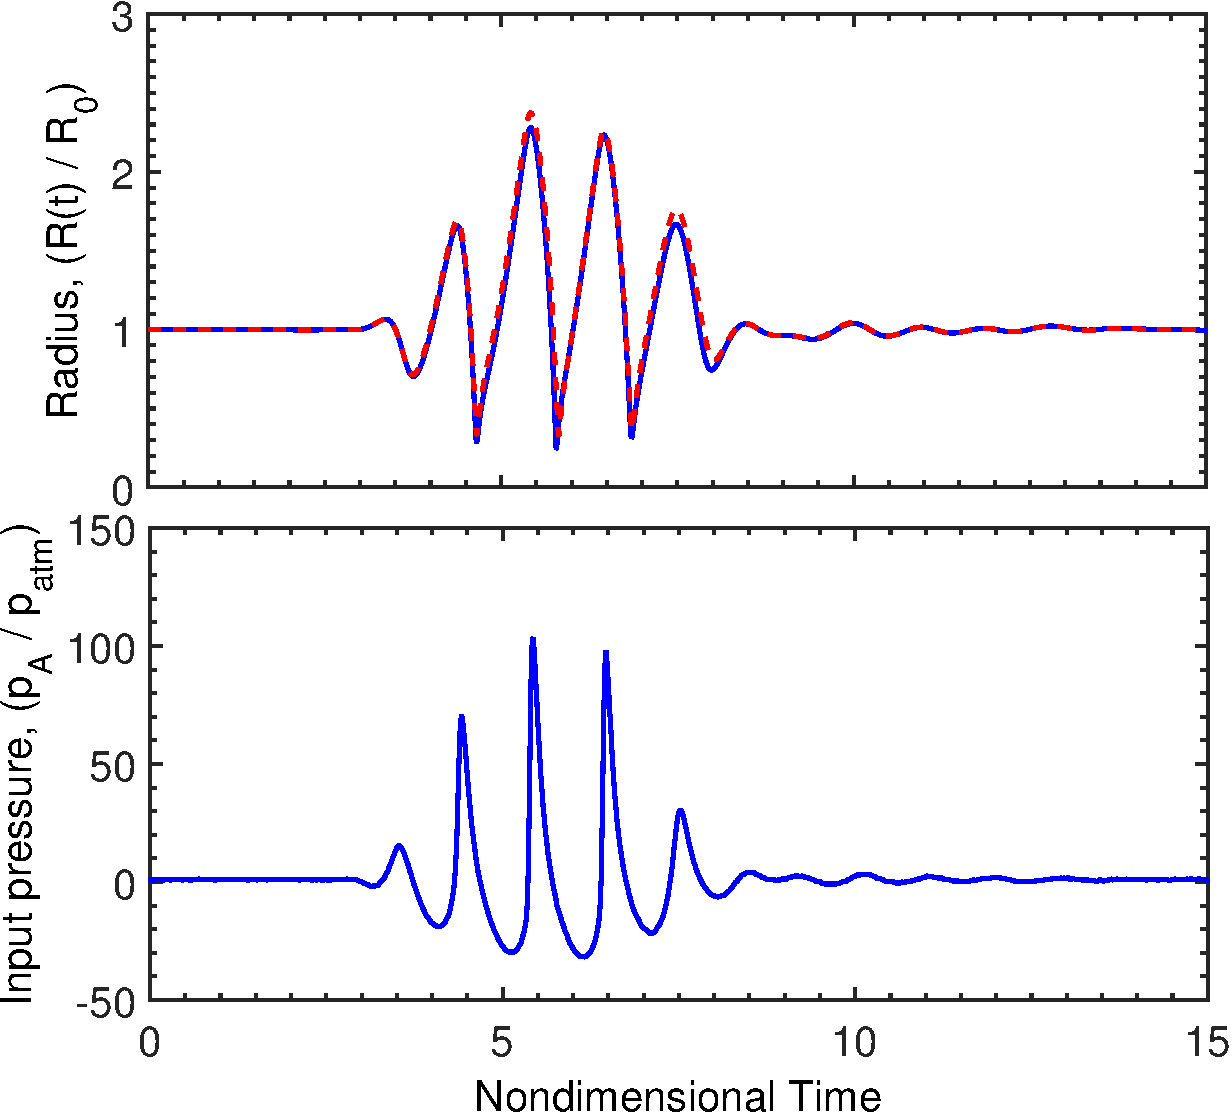
\includegraphics[width=\textwidth]{figs/bubble_figs/PFPair}
    \caption[History of the bubble radius for PFP and air]{}
    \label{fig:usbe_bubble_pfpair_radius}
  \end{subfigure}
  % 
  \begin{subfigure}{0.47\textwidth}
    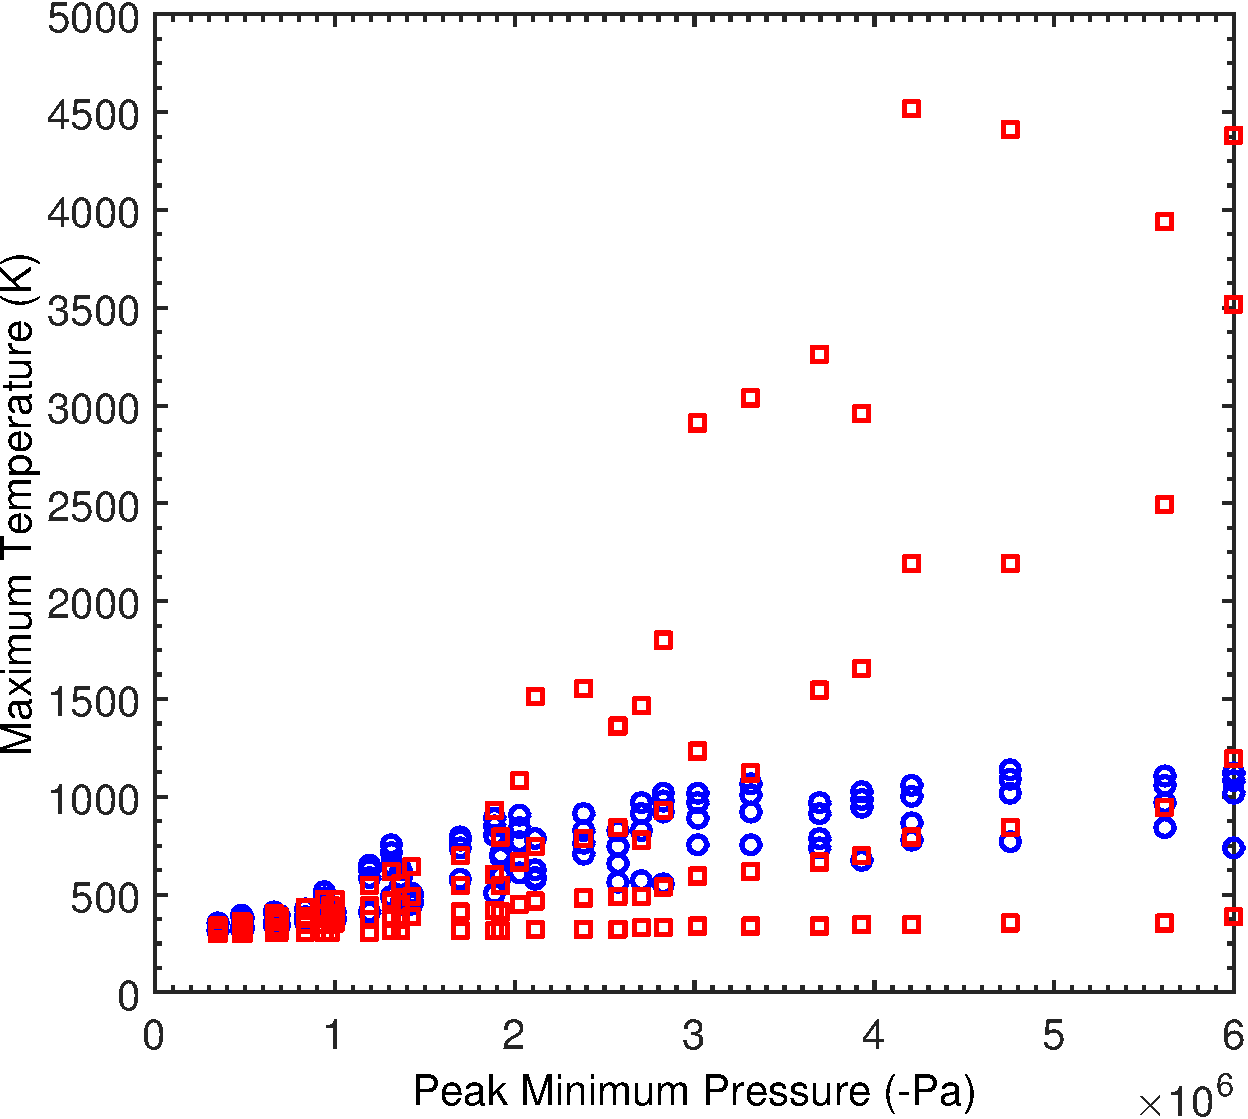
\includegraphics[width=\textwidth]{figs/bubble_figs/TmaxPFPair}
    \caption[Maximum temperature for PFP and air]{}
    \label{fig:usbe_bubble_pfpair_temp}
  \end{subfigure}
  \caption[Dependence of the bubble dynamics on the gas contents
  ($G=100$ kPa).]{Dependence of the bubble dynamics on the gas
    contents ($G=100$ kPa). \subref{fig:usbe_bubble_pfpair_radius}
    History of the bubble radius for PFP (solid) and air
    (dashed). $R_0=1$ $\mu$m; frequency: 3.5 MHz; peak negative
    pressure: 3.3 MPa. \subref{fig:usbe_bubble_pfpair_temp} Maximum
    temperature for PFP (circles) and air (squares). $R_0=0.1-2$
    $\mu$m; frequency: 1.5 - 7.5 MHz.}
  \label{fig:gascontents}
\end{figure}


\subsection{Dependence on the Initial (Equilibrium) Bubble Radius}

In the experiment, the size distribution of the UCAs is not known
exactly. It is desirable to know whether the observed bioeffects are
caused by all bubbles responding to the ultrasound, or whether a
specific size is more likely to be responsible at the bioeffects
threshold. To answer this question, for each experimental frequency,
bubbles of different radii ranging from 0.1--2 $\mu$m are subjected to
the pressure waveform corresponding to the bioeffects threshold
amplitude. It should be noted that varying the equilibrium radius
changes the non-dimensional parameters. Figure \ref{fig:size} shows the maximum dimensionless
radius, for both water (zero elasticity) and tissue (finite
elasticity, $G=100$ kPa), for the amplitude at which bioeffects are
first observed at a given frequency.

\begin{figure}[t]
  \centering
  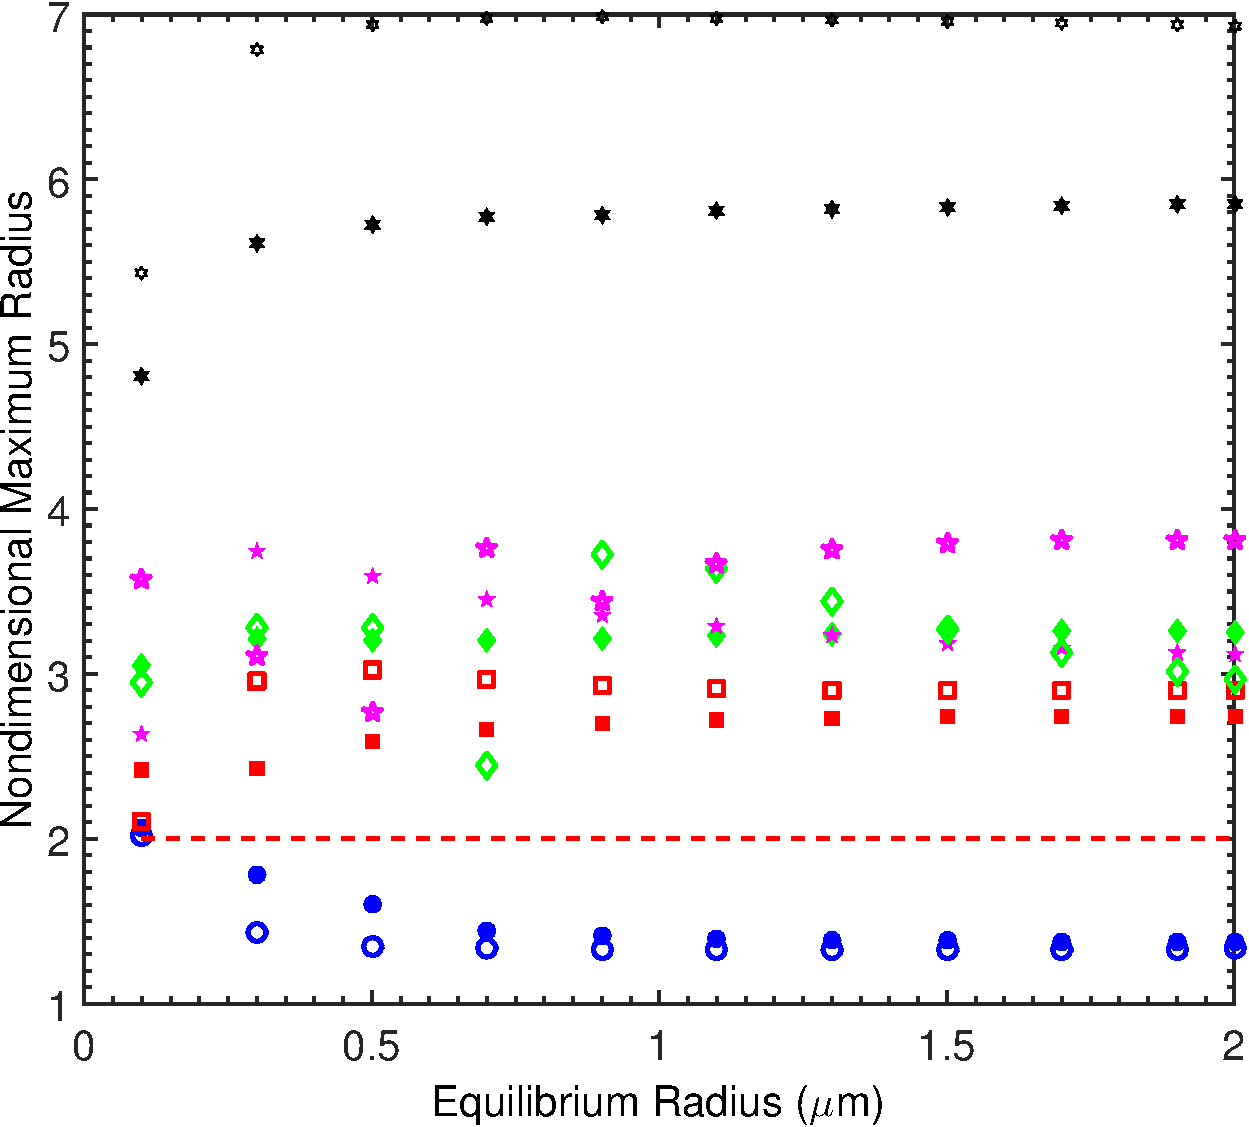
\includegraphics[width=.47\textwidth]{figs/bubble_figs/Rstarmax_R0}
  \caption[Dependence of the dimensionless maximum bubble radius on
  the initial bubble size for the amplitude at which bioeffects are
  first observed, at a given frequency, for $G=100$ kPa]{Dependence of
    the dimensionless maximum bubble radius on the initial bubble size
    for the amplitude at which bioeffects are first observed, at a
    given frequency, for $G=100$ kPa. Empty symbols: water; filled
    symbols: tissue. Circles: 1.50 MHz; squares: 2.25 MHz; diamonds:
    3.50 MHz; pentagrams: 5.00 MHz; hexagrams: 7.50 MHz. The
    $R_{max}=2$ inertial cavitation threshold (red, dashed line).}
  \label{fig:size}
\end{figure}

Excluding the smallest size, the bubble response in tissue is monotone
and changes little for a given frequency; there is no initial size
that consistently leads to a dramatic response. The somewhat erratic
behavior of the small bubbles may imply that such sizes are not
exclusively present in UCA concentrations. On the other hand, the
behavior is more irregular for water, particularly at small radii: for
a given frequency, there is an optimal size that exhibits the largest
response; these variations are much larger than for tissue.


 \subsection{Dependence on the Pulse Frequency}

The dependence of the bubble response on the pulse frequency is
considered in this section.  Figure \ref{fig:freq} shows the maximum
dimensionless and dimensional radius for all initial bubble sizes and
amplitudes vs. frequency. The square symbols denote cases in which
bioeffects were observed in the experiments, while the circular symbols
represent no bioeffects. The initial bubble sizes are not
discriminated here for simplicity.


\begin{figure*}[t]
  \centering
  \begin{subfigure}{0.47\textwidth}
    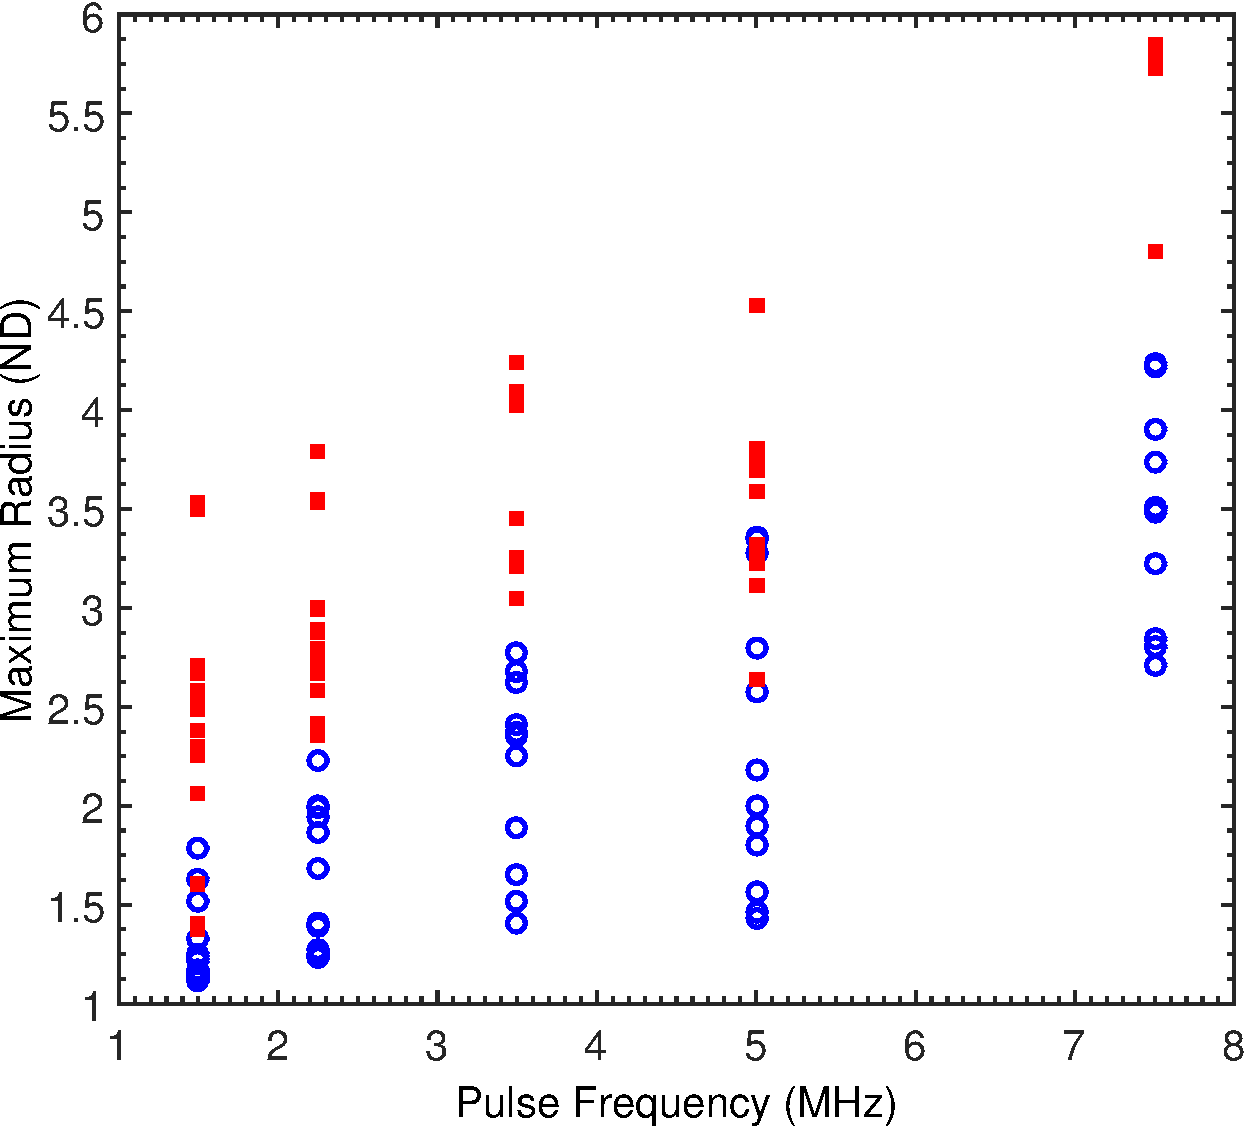
\includegraphics[width=\textwidth]{figs/bubble_figs/Rstarmax_F}
    \caption[Dependence of maximum dimensionless bubble radius on pulse frequency]{$R_{max}/R_0$}
    \label{fig:usbe_bubble_ndradius_frequency}
  \end{subfigure}  
  ~
  \begin{subfigure}{0.47\textwidth}
    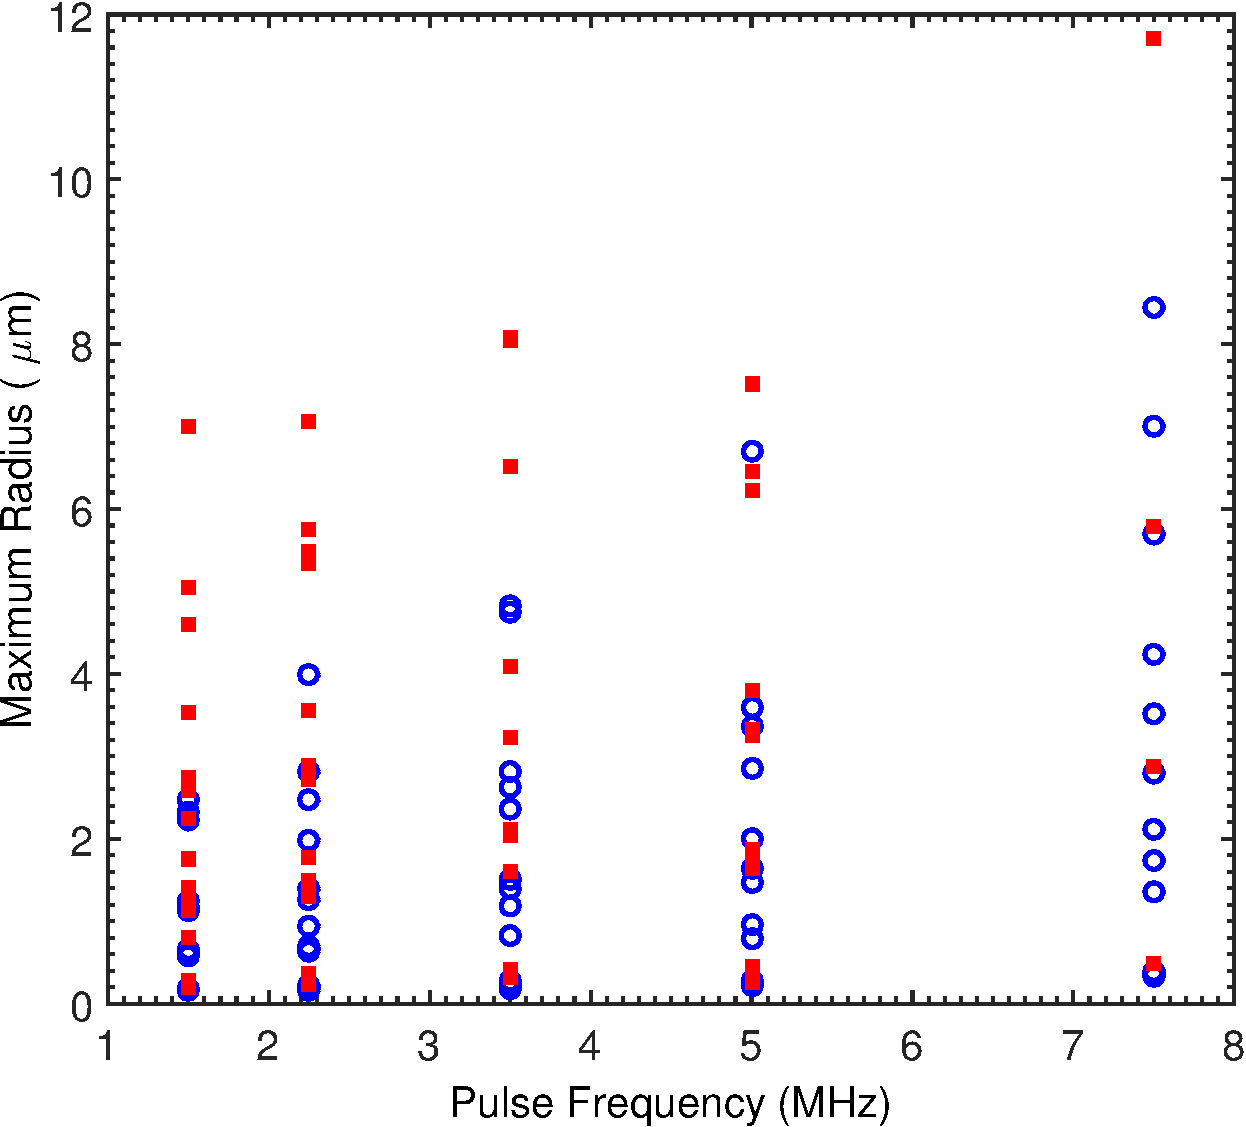
\includegraphics[width=\textwidth]{figs/bubble_figs/rmax_F}
    \caption[Dependence of maximum dimensional bubble radius on pulse frequency]{$R_{max}$}
    \label{fig:usbe_bubble_dradius_frequency}
  \end{subfigure}  
  \caption[Dependence of the bubble dynamics on the frequency for
    $G=100$ kPa]{Dependence of the bubble dynamics on the frequency for
    $G=100$ kPa. $R_0=0.1-2$ $\mu$m; empty circles: no bioeffects;
    squares: bioeffects. \subref{fig:usbe_bubble_ndradius_frequency}
    Dimensionless maximum bubble
    radius. \subref{fig:usbe_bubble_dradius_frequency} Dimensional
    maximum bubble radius.}
  \label{fig:freq}
\end{figure*}

With the exception of a few outliers, a clear separation between cases
for which bioeffects did and did not occur is observed; in other
words, the bioeffects threshold has a strong dependence on the
frequency. The trend appears to be approximately linear with
frequency. Large growth may be achieved with no evident bioeffects,
especially at high frequencies. The quantity $R_{max}$ is a
measure of cavitation collapse, since it is related to the available
energy of the bubble. Thus, the present results indicate that
cavitation collapse is expected to play an important role regarding
bioeffects, although the precise mechanism cannot be inferred.  Again,
the existing criteria for inertial cavitation thresholds are
frequency-independent and do not correlate well with the bioeffects
threshold, which clearly shows a strong dependence on frequency.

Another hypothesis is that bubble growth may be responsible for
capillary breaching. However, the plot of the dimensional maximum
radius vs. frequency does not show systematic bioeffects beyond a
certain size, \emph{e.g.}, some capillary diameter. Thus, growth is
not the sole mechanism by which bioeffects occur. However, the data
remains inconclusive, due to the inability to identify the cases in
which cavitation collapse is the dominant effect.






\subsection{Dependence on the Tissue Properties}
\label{sec:usbe_bubble_tissue_properties}

As suggested in
Figures \ref{fig:sample_bubble_linear}-\ref{fig:sample_bubble_nonlinear},
the bubble dynamics are sensitive to the tissue properties,
specifically the elasticity. However, different types of tissue may
have very different properties. Many of the measurements of tissue elasticity are made
\emph{in vitro}, and depend strongly on tissue preparation, storage,
and degradation as well as method of measurement.  Consequently, it is
possible that these measurements do not accurately represent the
current behavior.  To explore the effect of the elasticity on the
results and the correlation to bioeffects, Figure \ref{fig:freq_tissue}
shows the maximum dimensionless radius for all initial bubble sizes
and amplitudes vs. frequency for $G=5$ kPa and $G=1$ MPa. Although
seemingly high, the latter elasticity is chosen to match the work of
\cite{Yang2005}.

\begin{figure*}[t]
  \begin{subfigure}{0.47\textwidth}
    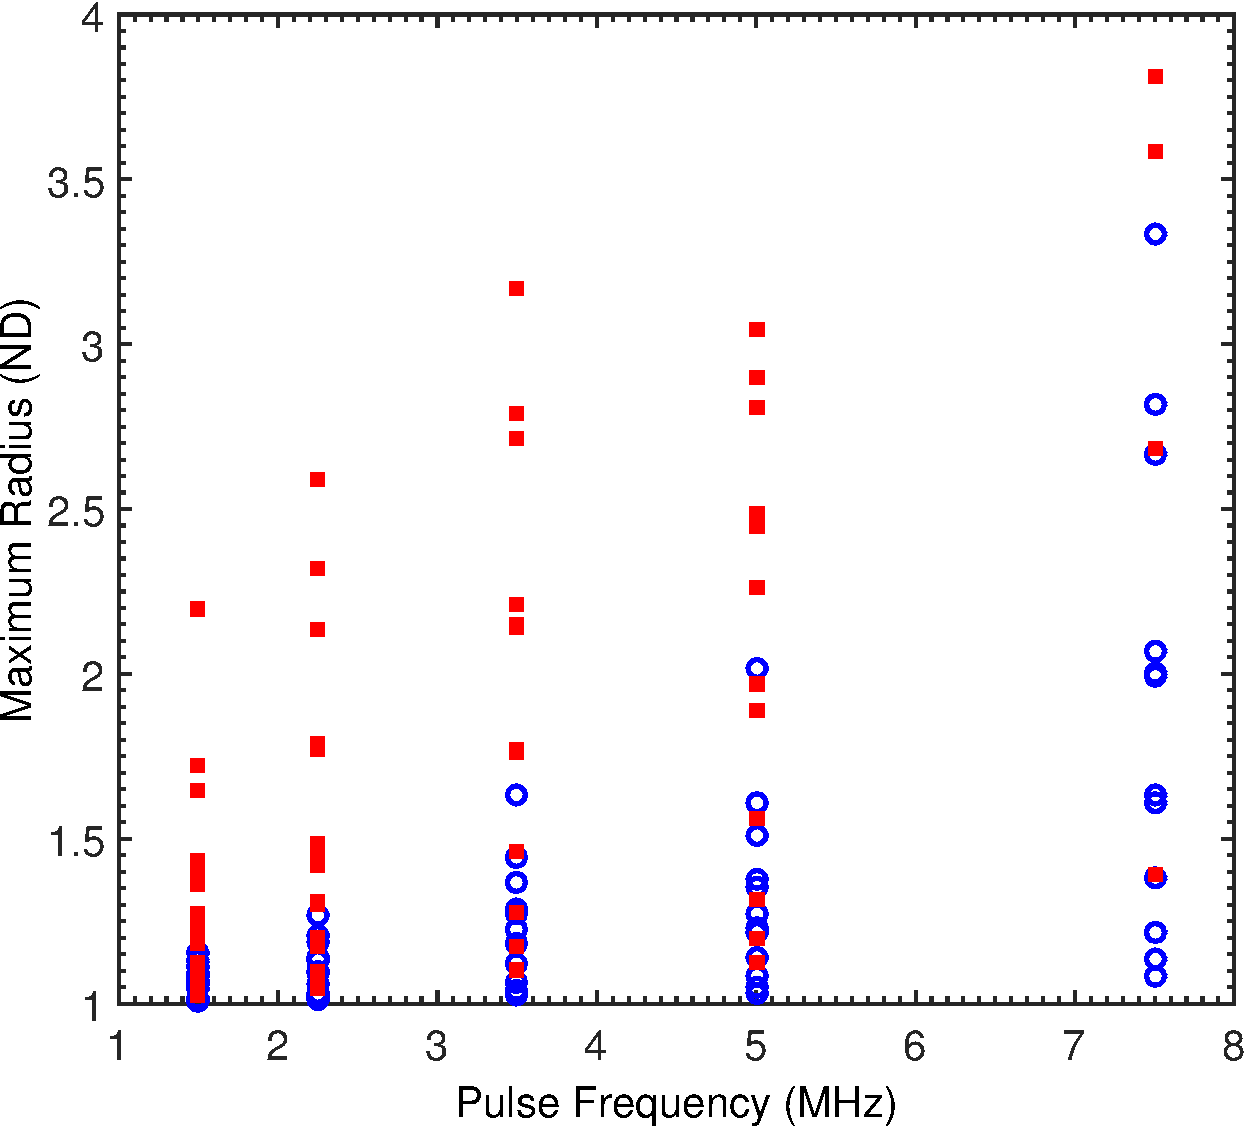
\includegraphics[width=\textwidth]{figs/bubble_figs/Rstarmax_F_Ca=20}
    \caption{$G=5$ kPa.}
  \label{fig:freq_tissue_Ca20}
  \end{subfigure}
  ~
  \begin{subfigure}{0.47\textwidth}
    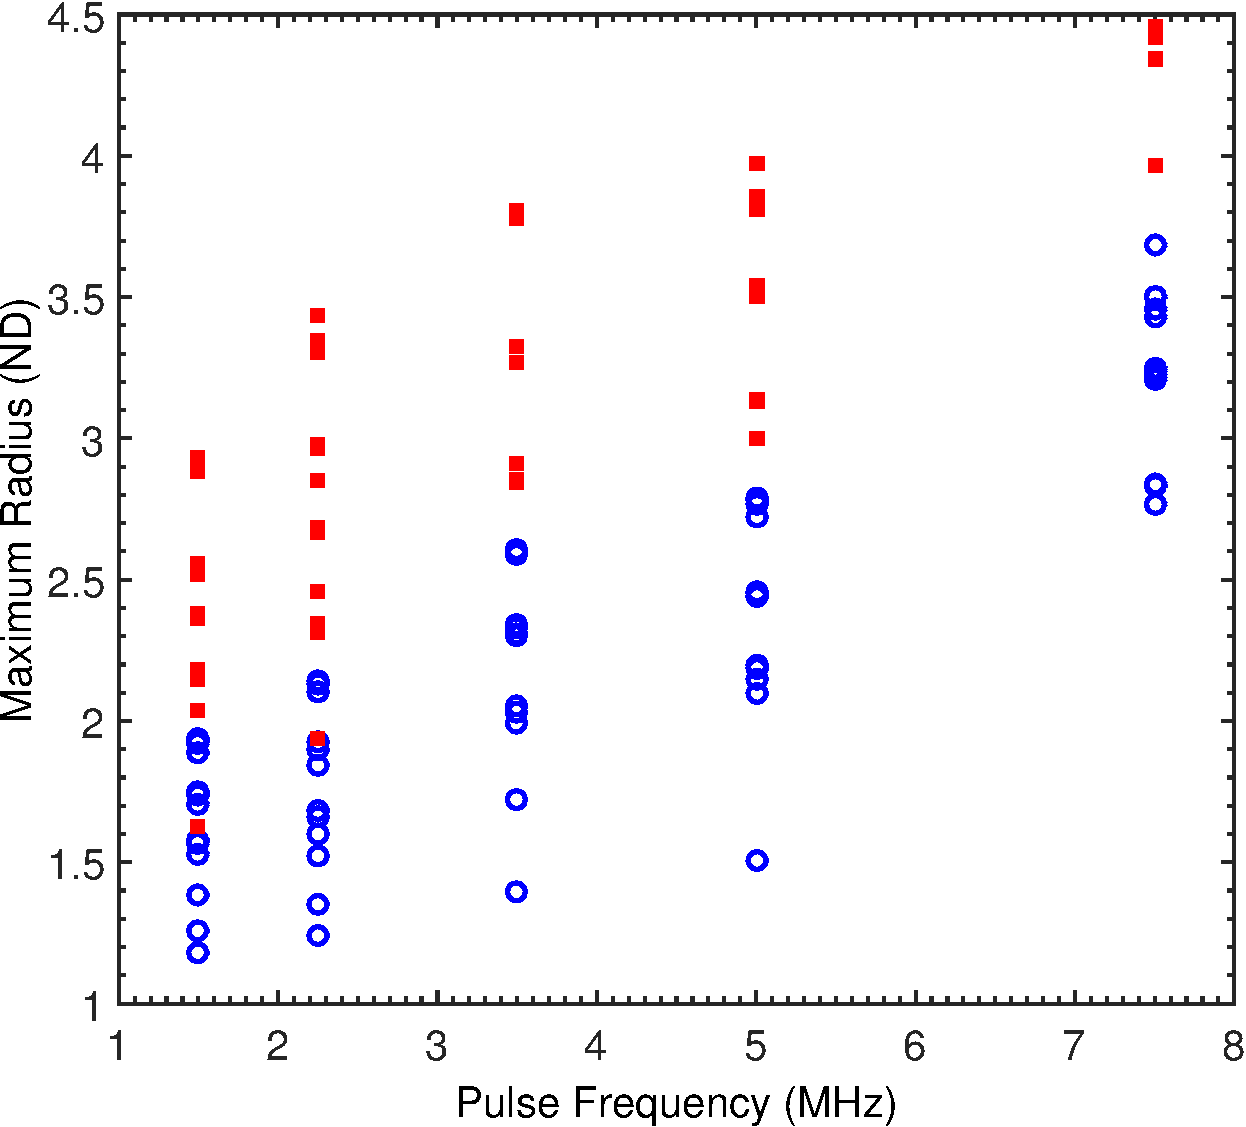
\includegraphics[width=\textwidth]{figs/bubble_figs/Rstarmax_F_Ca=0,1}
    \caption{$G=1$ MPa.}
    \label{fig:freq_tissue_Ca0,1}
  \end{subfigure}
  \caption[Dependence of the dimensionless maximum bubble
    radius on the frequency.]{Dependence of the dimensionless maximum bubble
    radius on the frequency. $R_0=0.1-2$ $\mu$m; empty circles: no
    bioeffects; squares: bioeffects. \subref{fig:freq_tissue_Ca20}
    $G=5$ kPa. \subref{fig:freq_tissue_Ca0,1} $G=1$ MPa.}
  \label{fig:freq_tissue}
\end{figure*}

The bubble dynamics and correlation to bioeffects significantly change
when reducing the elasticity. For a value of 5 kPa, the discrimination
is no longer clear. The bubble dynamics are closer to the behavior in
water, such that different sizes may have dramatically different
responses to the same waveform, as explained previously. On the other
hand, the stiffer medium ($G=1$ MPa) shows an even sharper
demarcation, which again appears to be approximately linear. Given the
sensitivity of the results on the elasticity, it is clear that more
precise \emph{in vivo} data is required for elasticities of tissues at the
relevant strain rates. 

Although not shown here, the type of
viscoelastic model significantly affects the bubble dynamics
\cite[]{Johnsen2012,Patterson2012}. For instance, a standard linear solid
model, which includes stress relaxation in addition to elasticity, leads 
to very different maximum
radii and oscillation properties (frequency and damping).  For
large relaxation times, elasticity variations become negligible.


% %%%%%%%%%%%%%%%%%%%%%%%%%%%%%%%%%%%%%%%%%%%%%%%%%%%%%%%%%%%%%%%%%%%%%%%%%%%%%%%%%%%%%%%%%%%%


\section{Conclusions}
\label{sec:usbe_bubble_conclusions}

In the present work, a numerical model is used to investigate
experimentally observed bioeffects as a result of contrast-enhanced
ultrasound. This work is unique in its combination of experimental
results and numerical modeling.  For the experimentally generated
input pressure waveforms, it is known which of these triggered
bioeffects, and from the numerical model we obtained calculated values
for the dimensionless maximum radius and dimensional maximum
temperature for each of these cases.  By comparing the results of this
study to previously established inertial cavitation thresholds used by
\cite{Apfel1991} and \cite{Yang2005}, $T_{max}=5000$ K and
$R_{max}=2$, it would appear that the inertial cavitation threshold
does not play a role in determining the bioeffects threshold.
However, it is unlikely that the inertial cavitation threshold is
irrelevant. Instead, it is far more probable that these thresholds are
not defined appropriately for cavitation in a viscoelastic medium,
such as soft tissue. This work suggests the need for further
experimental and numerical studies of cavitation in viscoelastic
media.

The present work shows a strong correlation between cavitation
dynamics and bioeffects when considering the pulse frequency.  From
the plot of maximum dimensionless radius vs. frequency, there is a
clear separation between when bioeffects do and do not occur, and
based on these results it appears that the frequency of the input
pressure waveforms is of key importance to the definition of a
bioeffect threshold, and likely the inertial cavitation threshold as
well.

The present work shows that the elasticity of tissue significantly
affects the bubble dynamics. This finding is perhaps not completely
unexpected given that bubble dynamics are known to strongly depend on
viscoelastic properties and model. The present study shows the need
for more accurate measurements of material properties and for
determining appropriate constitutive models for soft tissue,
particularly at high strain rates. Finally, although the present work
suggests that inertial cavitation collapse plays an important role
with respect to bioeffects, it does not shed light on the exact
mechanism, \emph{e.g.}, shock emission upon collapse, growth beyond a
given size, high temperatures generating free radicals, re-entrant
jets in non-spherical collapse, etc.  In future work we plan on
investigating this injury mechanism by conducting direct simulations
of the full equations of motion for bubble dynamics in a viscoelastic
medium.











%%%%%%%%%%%%%%%%%%%%%%%%%%%%%%%%%%%%%%%%%%%%%%%%%%%%%%%%%%%%%%%%%%





















% \begin{figure}
%   \centering \includegraphics[width=0.66\textwidth]{./figs/bubble_figs/rt_linear}
%   \caption{History of the bubble radius (top) and input-pressure
%     waveform (bottom) for an essentially linear case (frequency: 1.5 MHz; peak y
%     negative pressure: 0.35 MPa). No bioeffects are observed
%     here. $R_0=1$ $\mu$m; solid: $G=5$ kPa; dashed: $G=100$ kPa; dotted: $G=1$ MPa.}
%   \label{figure:sample_bubble_linear}
% \end{figure}

% \begin{figure}
%   \centering 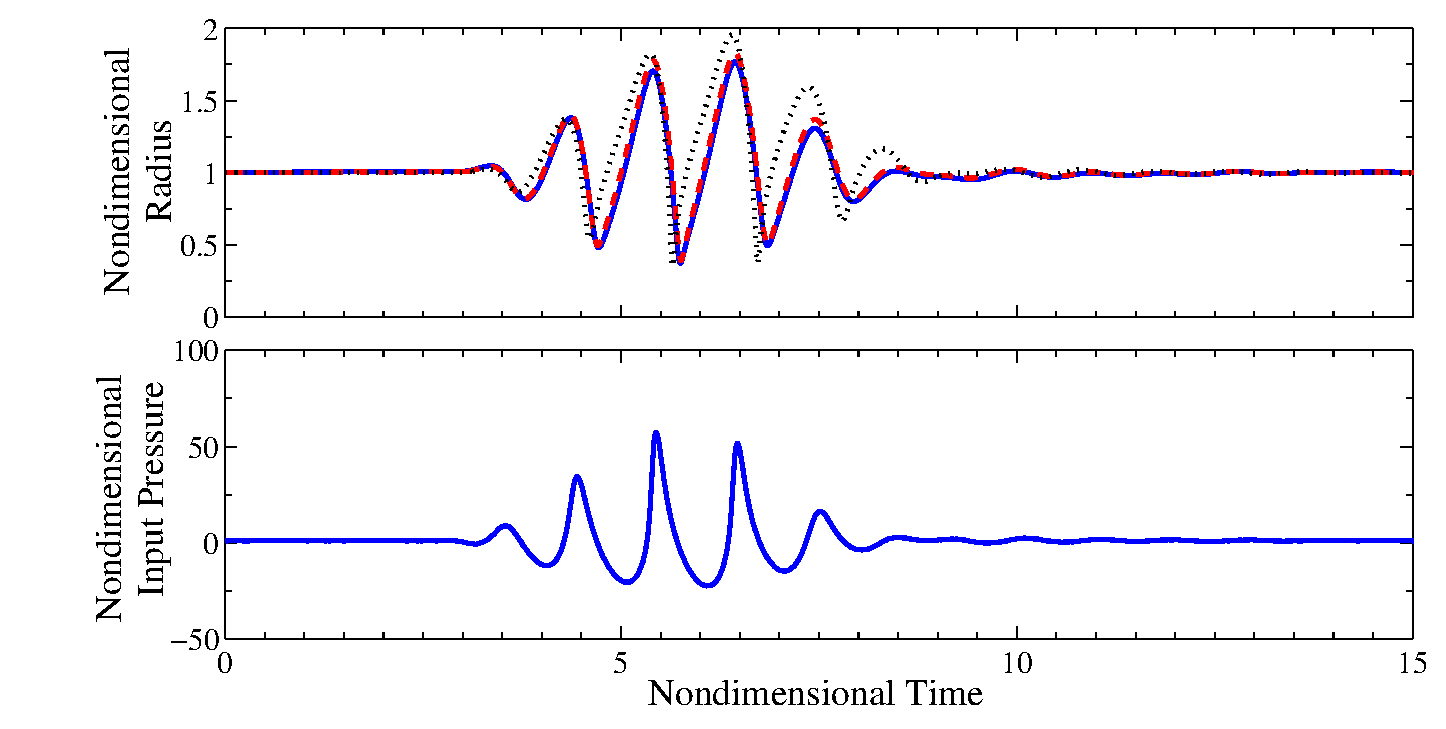
\includegraphics[width=0.66\textwidth]{./figs/bubble_figs/rt_intermediate}%
%   \caption{History of the bubble radius (top) and input-pressure
%     waveform (bottom) for a moderately nonlinear case (frequency: 3.5 MHz; peak 
%     negative pressure: 2.4 MPa). Bioeffects are
%     observed here. $R_0=1$ $\mu$m; solid: $G=5$ kPa; dashed: $G=100$ kPa;
%     dotted: $G=1$ MPa.}
%   \label{figure:sample_bubble_intermediate}
% \end{figure}

% \begin{figure}
%   \centering \includegraphics[width=0.66\textwidth]{./figs/bubble_figs/rt_nonlinear}
%   \caption{History of the bubble radius (top) and input-pressure
%     waveform (bottom) for a highly nonlinear case (frequency: 
%     7.5 MHz; peak negative pressure: 6.0 MPa). Bioeffects are observed
%     here. $R_0=1$ $\mu$m; solid: $G=5$ kPa; dashed: $G=100$ kPa; dotted: $G=1$ MPa.}
%   \label{figure:sample_bubble_nonlinear}
% \end{figure}

% In the results of the following sections, the maximum dimensionless radius,
% $R_{max}$, and dimensional bubble temperature at collapse, $T_{max}$, obtained
% using the ideal gas law, are determined by recording their largest
% value over the simulation. These quantities are compared to the
% inertial cavitation thresholds used by \cite{Apfel1991} and
% \cite{Yang2005}: $R_{max}=2$ and $T_{max}=5000$ K. The dependence
% of the bubble dynamics on the pulse amplitude, initial
% bubble size (\emph{i.e.}, UCA size distribution), 
% pulse frequency, and tissue properties are considered
% individually. 



% \subsection{Dependence on the Pulse Amplitude}

% Given the strong dependence of the MI on the rarefactional pressure
% amplitude, the influence of the pulse amplitude on the bubble dynamics
% is first evaluated. Figure ~\ref{figure:amplitude} shows the dimensionless
% maximum radius as a function of rarefactional pressure
% amplitude. Initial bubble radii ranging between 0.1--2.0 $\mu$m are
% shown, as well as different frequencies. The open symbols denote
% cases where bioeffects did not occur, while the filled symbols denote
% the occurrence of bioeffects.

% \begin{figure}[t]
%   \includegraphics[width=\columnwidth]{./figs/bubble_figs/rstarmax_pm}
%   \caption{(color online) Dependence of the dimensionless maximum bubble radius on
%     the peak negative pressure for $G=100$ kPa.  Empty symbols: no
%     bioeffects; filled symbols: bioeffects. Pentagrams: 0.1 $\mu$m; circles:
%     0.5 $\mu$m; squares: 1 $\mu$m; diamonds: 2 $\mu$m; frequency: 1.5 - 7.5 MHz. }
%   \label{figure:amplitude}
% \end{figure}

% The results show that the bubble dynamics, through the maximum radius,
% scale with the pulse amplitude. Although the results do not collapse fully
% onto a line, a general trend is discernible. At low amplitude, the increase in
% the maximum radius is approximately linear; beyond some amplitude, the bubble undergoes
% nonlinear oscillations, thus explaining the different depenced and larger spread. 
% These results are consistent with the plots shown in 
% Figs.~\ref{figure:sample_bubble_linear}-\ref{figure:sample_bubble_nonlinear}.
% Over a broad range of amplitudes, the
% occurrence of bioeffects has little correlation with pulse amplitude
% alone: at a given amplitude, bioeffects may be observed or not,
% depending on the bubble size and pulse frequency.  Only at very large
% pressure amplitudes (PRPA $>$ 4.20 MPa) are bioeffects systematically observed regardless of the
% bubble size and pulse frequency. This behavior is not surprising, since at
% these amplitudes the bubble response is expected to be highly
% nonlinear. Conversely, at low amplitudes (PRPA $<$ 0.97 MPa), the oscillations are 
% linear and no bioeffects are observed, regardless of
% bubble size and pulse frequency. In this latter case, most bubbles
% whose $R_{max}/R_0$ is below two do not exhibit bioeffects; however,
% this behavior depends on the value of elasticity, as shown in Section
% \ref{section:tissue_properties}.  Although not shown here for conciseness,
% similar results are obtained for peak positive pressure.


% Similarly, the criterion $T_{max} > 5000$ K is not achieved with perfluoropropane.
% As shown in Figure ~\ref{figure:gascontents}, the observed temperatures for
% PFP are far below this value, though the results for air approach it. This
% result is expected since the criterion was determined for air, which
% has a larger specific heats ratio ($\gamma_{air}=1.4$) than
% PFP ($\gamma= 1.13$). The specific heats ratio appears in
% the internal gas pressure term in Eq.~\ref{eq:bubble_pressure}; its
% effect on the bubble dynamics is minor if the minimum radius is not
% very small, as in Figure ~\ref{figure:gascontents}. Still, since the
% adiabatic relationships for an ideal gas are used, the temperature is
% significantly affected by the different specific heats ratio. Hence,
% even though the bubble dynamics are not strongly affected by the
% specific heats ratio, the maximum temperature is.

% \begin{figure*}[t]
%   \begin{subfigure}[b]{0.47\textwidth}
%   \includegraphics[width=\textwidth]{./figs/bubble_figs/pfpair}
%   \caption{History of the bubble radius for PFP (solid) and air
%     (dashed). $R_0=1$ $\mu$m; frequency: 3.5 MHz; peak negative
%     pressure: 3.3 MPa}
% \end{subfigure}
%   \begin{subfigure}[b]{0.47\textwidth}
%     \includegraphics[width=\textwidth]{./figs/bubble_figs/tmaxpfpair} 
%     \caption{Maximum temperature for PFP (circles) and air (squares). $R_0=0.1-2$ $\mu$m; frequency: 1.5 - 7.5 MHz.}
%   \end{subfigure}
%   \caption{(color online) Dependence of the bubble dynamics on the gas contents ($G=100$ kPa).}
%   \label{figure:gascontents}
% \end{figure*}

% % \begin{figure*}[t]
% %   \subfigure[History of the bubble radius for PFP (solid) 
% %     and air (dashed). $R_0=1$ $\mu$m; frequency: 3.5 MHz; peak negative pressure: 3.3 MPa]{
% %   \includegraphics[width=0.47\textwidth]{./figs/bubble_figs/pfpair} }
% %   \subfigure[Maximum temperature for PFP (circles) and air (squares). $R_0=0.1-2$ $\mu$m; frequency: 1.5 - 7.5 MHz. ]{
% %   \includegraphics[width=0.47\textwidth]{./figs/bubble_figs/tmaxpfpair} }
% %   \caption{(color online) Dependence of the bubble dynamics on the gas contents
% %   ($G=100$ kPa).}
% %   \label{figure:gascontents}
% % \end{figure*}






% \subsection{Dependence on the Initial (Equilibrium) Bubble Radius}

% In the experiment, the size distribution of the UCAs is not known
% exactly. It is desirable to know whether the observed bioeffects are
% caused by all bubbles responding to the ultrasound, or whether a
% specific size is more likely to be responsible at the bioeffects
% threshold. To answer this question, for each experimental frequency,
% bubbles of different radii ranging from 0.1--2 $\mu$m are subjected to
% the pressure waveform corresponding to the bioeffects threshold
% amplitude. It should be noted that varying the equilibrium radius
% changes the non-dimensional parameters. Figure ~\ref{figure:size} shows the maximum dimensionless
% radius, for both water (zero elasticity) and tissue (finite
% elasticity, $G=100$ kPa), for the amplitude at which bioeffects are
% first observed at a given frequency.

% \begin{figure}[t]
%     \includegraphics[width=\columnwidth]{./figs/bubble_figs/rstarmax_r0}
%     \caption{(color online) Dependence of the dimensionless maximum bubble radius on
%       the initial bubble size for the amplitude at which bioeffects
%       are first observed, at a given frequency, for $G=100$ kPa. Empty
%       symbols: water; filled symbols: tissue. Circles: 1.50 MHz; squares:
%       2.25 MHz; diamonds: 3.50 MHz; pentagrams: 5.00 MHz; hexagrams: 7.50 MHz.}
%     \label{figure:size}
% \end{figure}

% Excluding the smallest size, the bubble response in tissue is monotone
% and changes little for a given frequency; there is no initial size
% that consistently leads to a dramatic response. The somewhat erratic
% behavior of the small bubbles may imply that such sizes are not
% present in UCA concentrations. On the other hand, the behavior is more
% irregular for water, particularly at small radii: for a given
% frequency, there is an optimal size that exhibits the largest
% response; these variations are much larger than for tissue.  








% \subsection{Dependence on the Pulse Frequency}

% The dependence of the bubble response on the pulse frequency is
% considered in this section.  Figure ~\ref{figure:freq} shows the maximum
% dimensionless and dimensional radius for all initial bubble sizes and
% amplitudes vs. frequency. The square symbols denote cases in which
% bioeffects were observed in the experiments, while the circular symbols
% represent no bioeffects. The initial bubble sizes are not
% discriminated here for simplicity.


% \begin{figure*}[t]
%   \begin{subfigure}[b]{0.47\textwidth}
%     \includegraphics[width=\textwidth]{./figs/bubble_figs/rstarmax_f}  
%     \caption{Dimensionless maximum bubble radius.}
%   \end{subfigure}

%   \begin{subfigure}[b]{0.47\textwidth}
%     \includegraphics[width=0.47\textwidth]{./figs/bubble_figs/rmax_f}      
%     \caption{Dimensional maximum bubble radius.}
%   \end{subfigure}
%   \caption{(color online) Dependence of the bubble dynamics on the frequency for
%     $G=100$ kPa. $R_0=0.1-2$ $\mu$m; empty circles: no bioeffects; squares:
%     bioeffects.}
%   \label{figure:freq}
% \end{figure*}

% With the exception of a few outliers, a clear separation between cases
% for which bioeffects did and did not occur is observed; in other
% words, the bioeffects threshold has a strong dependence on the
% frequency. The trend appears to be approximately linear with
% frequency. Large growth may be achieved with no evident bioeffects,
% especially at high frequencies. The quantity $R_{max}$ is a
% measure of cavitation collapse, since it is related to the available
% energy of the bubble. Thus, the present results indicate that
% cavitation collapse is expected to play an important role regarding
% bioeffects, although the precise mechanism cannot be inferred.  Again,
% the existing criteria for inertial cavitation thresholds are
% frequency-independent and do not correlate well with the bioeffects
% threshold, which clearly shows a strong dependence on frequency.

% Another hypothesis is that bubble growth may be responsible for
% capillary breaching. However, the plot of the dimensional maximum radius vs. frequency does
% not show systematic bioeffects beyond a certain size, \emph{e.g.},
% some capillary diameter. Thus, growth is not the sole mechanism by
% which bioeffects occur. However, the data remains inconclusive,
% due to the inability to identify the cases in which cavitation
% collapse is the dominant effect.






% \subsection{Dependence on the Tissue Properties}
% \label{section:tissue_properties}

% As suggested in
% Figs.~\ref{figure:sample_bubble_linear}-\ref{figure:sample_bubble_nonlinear},
% the bubble dynamics are sensitive to the tissue properties,
% specifically the elasticity. However, different types of tissue may
% have very different properties. Many of the measurements of tissue elasticity are made
% \emph{in vitro}, and depend strongly on tissue preparation, storage,
% and degradation as well as method of measurement.  Consequently it is
% possible that these measurements do not accurately represent the
% current behavior.  To explore the effect of the elasticity on the
% results and the correlation to bioeffects, Figure ~\ref{figure:freq_tissue}
% shows the maximum dimensionless radius for all initial bubble sizes
% and amplitudes vs. frequency for $G=5$ kPa and $G=1$ MPa. Although
% seemingly high, the latter elasticity is chosen to match the work of
% \cite{Yang2005}.

% \begin{figure*}[t]
%   \begin{subfigure}[b]{0.47\textwidth}
%     \includegraphics[width=\textwidth]{./figs/bubble_figs/rstarmax_f_ca=20}
%     \caption{$G=5$ kPa.}
%   \end{subfigure}

%   \begin{subfigure}[b]{0.47\textwidth}
%     \includegraphics[width=\textwidth]{./figs/bubble_figs/rstarmax_f_ca=0,1}    
%     \caption{$G=1$ MPa.}
%   \end{subfigure}
%   \caption{(color online) Dependence of the dimensionless maximum bubble radius on
%      the frequency. $R_0=0.1-2$ $\mu$m; empty circles: no bioeffects; squares:
%      bioeffects.}
%   \label{figure:freq_tissue}
% \end{figure*}

% % \begin{figure*}[t]
% %   \subfigure[$G=5$ kPa.]{
% %     \includegraphics[width=0.47\textwidth]{./figs/bubble_figs/rstarmax_f_ca=20}
% %   }
% %   \subfigure[$G=1$ MPa.]{
% %     \includegraphics[width=0.47\textwidth]{./figs/bubble_figs/rstarmax_f_ca=0,1}    
% %   }
% %    \caption{(color online) Dependence of the dimensionless maximum bubble radius on
% %      the frequency. $R_0=0.1-2$ $\mu$m; empty circles: no bioeffects; squares:
% %      bioeffects.}
% %   \label{figure:freq_tissue}
% % \end{figure*}

% The bubble dynamics and correlation to bioeffects significantly change
% when reducing the elasticity. For a value of 5 kPa, the discrimination
% is no longer clear. The bubble dynamics are closer to the behavior in
% water, such that different sizes may have dramatically different
% responses to the same waveform, as explained previously. On the other
% hand, the stiffer medium ($G=1$ MPa) shows an even sharper
% demarcation, which again appears to be approximately linear. Given the
% sensitivity of the results on the elasticity, it is clear that more
% precise \emph{in vivo} data is required for elasticities of tissues at the
% relevant strain rates. 

% Although not shown here, the type of
% viscoelastic model significantly affects the bubble dynamics
% \cite[]{Johnsen2012}. For instance, a standard linear solid
% model, which includes stress relaxation in addition to elasticity, leads 
% to very different maximum
% radii and oscillation properties (frequency and damping).  For
% large relaxation times, elasticity variations become negligible.




% \section{Conclusions}
% \label{sec:usbe_bubble_conclusions}

% In the present work, a numerical model is used
% to investigate experimentally observed bioeffects as a result of
% contrast-enhanced ultrasound. This work is unique in its 
% combination of experimental results and numerical modeling.
% For the experimentally generated input
% pressure waveforms, it is known which of these triggered bioeffects,
% and from the numerical model we obtained calculated values for
% the dimensionless maximum radius and dimensional maximum temperature for each of these cases.  By comparing the
% results of this study to previously established inertial cavitation
% thresholds used by \cite{Apfel1991} and \cite{Yang2005},
% $T_{max}=5000$ K and $R_{max}=2$, it would appear that the inertial
% cavitation threshold does not play a role in determining the bioeffects
% threshold.  However, it is unlikely that the inertial cavitation
% threshold is irrelevant. Instead, it is far more probable that these
% thresholds are not defined appropriately for cavitation in a
% viscoelastic medium, such as soft tissue. This work suggests the need for
% further experimental and numerical studies of cavitation in viscoelastic media.

% The present work shows a strong correlation between cavitation dynamics and bioeffects
% when considering the pulse frequency.
% From the plot of maximum
% dimensionless radius vs. frequency, there is a clear separation
% between when bioeffects do and do not occur, and based on these
% results it appears that the frequency of the input pressure waveforms
% is of key importance to the definition of a bioeffect threshold, and
% likely the inertial cavitation threshold as well. 

% The present work shows that the elasticity of tissue significantly
% affects the bubble dynamics. This finding is perhaps not completely
% unexpected given that bubble dynamics are known to strongly depend
% on viscoelastic properties and model. The present study shows the need
% for more accurate measurements of material properties and for
% determining appropriate constitutive models for soft tissue,
% particularly at high strain rates. Finally, although the present work
% suggests that inertial cavitation collapse plays an important role with respect
% to bioeffects, it does not shed light on the exact mechanism,
% \emph{e.g.}, shock emission upon collapse, growth beyond a given size,
% high temperatures generating free radicals, re-entrant jets in
% non-spherical collapse, etc.  In future work we plan on investigating 
% this injury mechanism by conducting direct simulations of
% the full equations of motion for bubble dynamics in a viscoelastic medium.


%%% Local Variables:
%%% mode: latex
%%% TeX-master: t
%%% End:
